\section{Lavoro svolto}
Il gruppo inizialmente ha deciso di adottare un metodo a cascata durante la stesura dei documenti iniziali e del way of working. 
Successivamente, con l'analisi dei requisiti e l'inizio della codifica, il gruppo ha adottato un metodo agile di tipo scrum al fine di organizzarsi meglio e preventivare in anticipo le attività da svolgere per raggiungere l'obiettivo prefissato.
Ogni sprint presenta le seguenti caratteristiche:
\begin{itemize}
    \item{Durata:} 2 settimane.
    \item{Attività svolte:} Attività che il gruppo si è prefissato e che ha portato a termine.
    \item{Difficoltà riscontrate:} A fine dello sprint, tramite un lavoro di retrospettiva si riflette sulle difficoltà incontrate.
    \item{Costi Previsti}
    \item{Costi Effettivi}
\end{itemize}

\subsection{Way of working}



\begin{longtable}{|p{0.085\textwidth}|c|c|c|c|c|c|c|p{0.07\textwidth}|}
    \hline
    Nome &\begin{tabular}[c]{@{}c@{}} dal 26/04\\ al 30/04 \end{tabular} & \begin{tabular}[c]{@{}c@{}}dal 01/05\\ al 04/05\end{tabular} & \begin{tabular}[c]{@{}c@{}}dal 04/05\\ al 12/05\end{tabular} & \begin{tabular}[c]{@{}c@{}}dal 13/05\\ al 19/05\end{tabular} & \begin{tabular}[c]{@{}c@{}}dal 20/05\\ al 26/05\end{tabular} & \begin{tabular}[c]{@{}c@{}}dal 27/5\\ al 03/06\end{tabular} & \begin{tabular}[c]{@{}c@{}}dal 04/06\\ al 09/06\end{tabular} & Totale ore\\
    \hline
    Ibra Elton & AN - 4 ore & VE - 2 ora& AN - 3 ore & RE - 3 ore & AN - 3 ore & VE -2 ore & PR - 4 ore  & 20\\
    \hline
    Beschin Michele & AN - 3 ore & AN - 3 ore & RE - 4 ore & AN - 2 ore & VE - 2 ore & AN - 4 ore & PR - 3 ore & 21 \\
    \hline
    Lotto Riccardo & AN - 3 ore & RE - 4 ore & AN - 3 ore & VE - 1 ore & AN - 4 ore & VE - 2 ore & PT - 3 ore & 20\\
    \hline
    Bobirica Andrei Cristian & AN - 4 ore & AN - 3 ore & VE - 1 ore & AN - 2 ore & VE - 2 ore & AN - 4 ore & RE - 5 ore & 22\\
    \hline
    Andreetto Alessio & AN - 3 ore & VE - 2 ore & AN - 3 ore & VE - 2 ore & AN - 4 ore & RE - 4 ore & AN - 3 ore & 21\\
    \hline
    Corbu Teodor Mihail & AN - 3 ore & AN - 4 ore & VE - 2 ore & AN - 2 ore & RE - 3 ore & AN - 3 ore & VE - 2 ore & 19\\
    \hline
\end{longtable}

\begin{longtable}{|c|c|}
    \hline
    \textbf{Legenda} & \\
    \hline
    RE & Responsabile \\
    \hline
    AN & Analista \\
    \hline
    VE & Verificatore \\
    \hline
    PR & Programmatore \\
    \hline
    PT & Progettista \\
    \hline
    AM & Amministratore \\
    \hline
\end{longtable}

\begin{longtable}{|p{0.085\textwidth}|c|c|c|c|c|c|c|}
    \hline
    Nome &\begin{tabular}[c]{@{}c@{}} dal 26/04\\ al 30/04 \end{tabular} & \begin{tabular}[c]{@{}c@{}}dal 01/05\\ al 04/05\end{tabular} & \begin{tabular}[c]{@{}c@{}}dal 04/05\\ al 12/05\end{tabular} & \begin{tabular}[c]{@{}c@{}}dal 13/05\\ al 19/05\end{tabular} & \begin{tabular}[c]{@{}c@{}}dal 20/05\\ al 26/05\end{tabular} & \begin{tabular}[c]{@{}c@{}}dal 27/5\\ al 03/06\end{tabular} & \begin{tabular}[c]{@{}c@{}}dal 04/06\\ al 09/06\end{tabular} \\
    \hline
    Ibra Elton & AN - 4 ore & VE - 2 ora& AN - 3 ore & RE - 3 ore & AN - 3 ore & VE -2 ore & PR - 4 ore  \\
    \hline
    Beschin Michele & AN - 3 ore & AN - 3 ore & RE - 4 ore & AN - 2 ore & VE - 2 ore & AN - 4 ore & PR - 3 ore  \\
    \hline
    Lotto Riccardo & AN - 3 ore & RE - 4 ore & AN - 3 ore & VE - 1 ore & AN - 4 ore & VE - 2 ore & PT - 3 ore\\
    \hline
    Bobirica Andrei Cristian & AN - 4 ore & AN - 3 ore & VE - 1 ore & AN - 2 ore & VE - 2 ore & AN - 4 ore & RE - 5 ore \\
    \hline
    Andreetto Alessio & AN - 3 ore & VE - 2 ore & AN - 3 ore & VE - 2 ore & AN - 4 ore & RE - 4 ore & AN - 3 ore \\
    \hline
    Corbu Teodor Mihail & AN - 3 ore & AN - 4 ore & VE - 2 ore & AN - 2 ore & RE - 3 ore & AN - 3 ore & VE - 2 ore\\
    \hline
    Ore settimanali & 20 &  18&  16&  12&  18&  19&  20 \\
    \hline 
    Costi preventivati & 525 € & 400 € & 430 € & 285 € & 470 € & 495 € & 470 € \\
    \hline
    Costi effettivi &  500 €& 450 € & 405 € & 300 €& 445 € & 475 € & 445 € \\
    \hline
\end{longtable}






\subsection{Requirements and technology baseline}
In vista della prima revisione RTB, il gruppo ha scelto di cambiare metodologia di lavoro. Per facilitare la stesura del codice, si è scelto di optare per una metodologia agile suddivisa in sprint.


\subsubsection{Sprint 1}
\begin{center}
    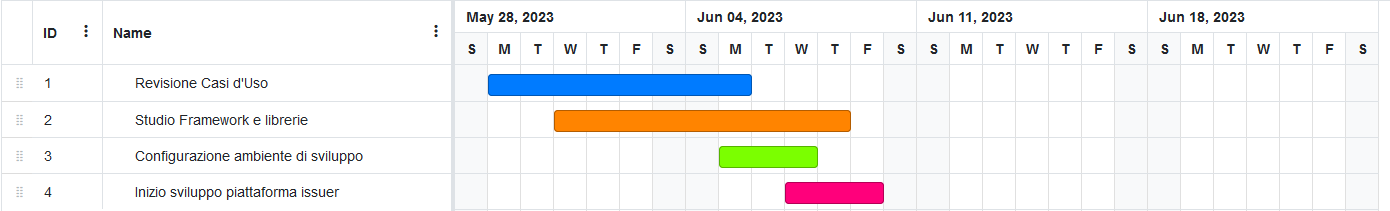
\includegraphics[scale = 0.4]{./res/img/Sprint_1.png}
  \end{center}

\begin{itemize}
\item \textbf{Durata:} 29/05/2023 - 09/06/2023 
\item \textbf{Attività svolte:}
\begin{itemize}
    \item Ampliamento e revisione della sezione "casi d'uso" all'interno del documento Analisi dei requisiti;
    \item Analisi e studio dei framework e librerie da utilizzare per lo sviluppo del codice;
    \item Creazione e configurazione dell'ambiente di sviluppo;
    \item Inizio sviluppo piattaforma issuer.
\end{itemize}
\item \textbf{Difficoltà riscontrate:}
\begin{itemize}
    \item Lo sviluppo della piattaforma holder non era compatibile parallelamente a quella issuer; 
    \item Difficoltà nel gestire tutte le istanze all'interno di Docker\glo, si è optato per mantenere su container docker soltanto le API.
\end{itemize}
\newpage
\item \textbf{Costi Previsti:}
\begin{longtable}{|c|c|c|c|}
    \hline
    Ruolo & Descrizione & Ore & Costo \\
    \hline
    RE & Responsabile & 5 & 150€ \\
    \hline
    AN & Analista & 5 & 125€ \\
    \hline
    VE & Verificatore & 5 & 100€ \\
    \hline
    PR & Programmatore & 8 & 120€ \\
    \hline
    PT & Progettista & 4 & 100€ \\
    \hline
    AM & Amministratore & 3 & 60€ \\
    \hline
    Totale & & 30 & 655€ \\
    \hline
    \end{longtable}
\item \textbf{Costi effettivi:}
\begin{longtable}{|p{0.1\textwidth}|c|c|c|c|c|c|c|c|}
    \hline
    Nome & RE & AN & VE & PR & PT & AM & Ore & Costi\\
    \hline
    Ibra Elton &5 & & & & & &5 & 150€\\
    \hline
    Beschin Michele & & & &4 & & &4 & 60€ \\
    \hline
    Lotto \newline  Riccardo & & & &5 & & &5& 75€ \\
    \hline
    Bobirica Andrei Cristian & & & & &3 &2 &5 & 115€\\
    \hline
    Andreetto Alessio & &6 & & & & &6 & 150€\\
    \hline
    Corbu Teodor Mihail & & &6 & & & &6 & 120€\\
    \hline
    Totale &5 &6 &6 &9 &3 &2 &31& 670€\\
    \hline
\end{longtable}
\end{itemize}

\subsubsection{Sprint 2}
\begin{center}
    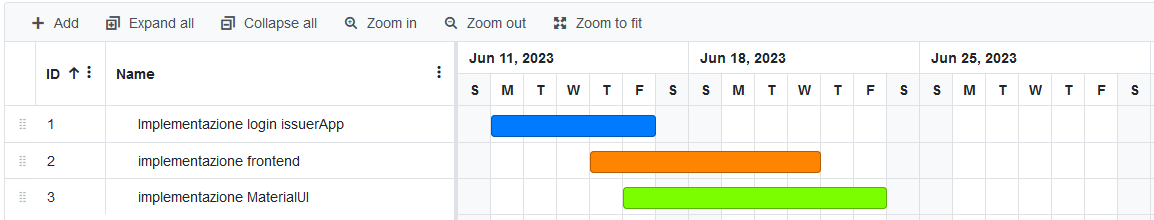
\includegraphics[scale = 0.45]{./res/img/Sprint_2.png}
  \end{center}

\begin{itemize}
    \item \textbf{Durata:} 12/06/2023 - 23/06/2023 
    \item \textbf{Attività svolte:}
    \begin{itemize}
        \item È stata implementata la libreria grafica Material UI su un branch separato;
        \item È stato implementato il sistema di login per issuer app; 
        \item Implementazione del front-end per la richiesta di credenziale nell'issuer.
    \end{itemize}
    \item \textbf{Difficoltà riscontrate:}
    \begin{itemize}
        \item Al momento attuale lo sviluppo del verifier non è compatibile parallelamente ad issuer.
    \end{itemize}
    \item \textbf{Costi Previsti:}
    \begin{longtable}{|c|c|c|c|}
        \hline
        Ruolo & Descrizione & Ore & Costo \\
        \hline
        RE & Responsabile & 4 & 120€ \\
        \hline
        AN & Analista & 0 & 0€ \\
        \hline
        VE & Verificatore & 3 & 60€ \\
        \hline
        PR & Programmatore & 13 & 195€ \\
        \hline
        PT & Progettista & 15 & 375€ \\
        \hline
        AM & Amministratore & 4 & 80€ \\
        \hline
        Totale & & 39 & 830€ \\
        \hline
        \end{longtable}
    \item \textbf{Costi effettivi:}
    \begin{longtable}{|p{0.1\textwidth}|c|c|c|c|c|c|c|c|}
        \hline
        Nome & RE & AN & VE & PR & PT & AM & Ore & Costi\\
        \hline
        Ibra \newline Elton & & & &6 & & &6 & 90€\\
        \hline
        Beschin Michele & & & & &7 & &7 & 175€\\
        \hline
        Lotto \newline Riccardo &2 & & & &5 & &7 & 185€\\
        \hline
        Bobirica Andrei Cristian & & & & &3 &4 &7 & 155€\\
        \hline
        Andreetto Alessio &2 & & &3 & & &5 & 105€\\
        \hline
        Corbu Teodor Mihail & & &3 &4 & & &7 & 120€\\
        \hline
        Totale &4 &0 &3 &13 &15 &4 &39 & 830€\\
 
        \hline
    \end{longtable}
    \end{itemize}

\subsubsection{Sprint 3}
\begin{center}
    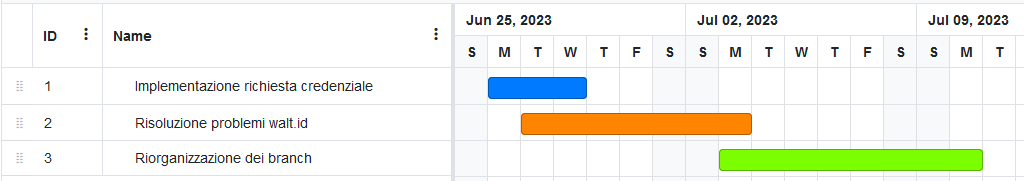
\includegraphics[scale = 0.5]{./res/img/Sprint_3.png}
  \end{center}
\begin{itemize}
    \item \textbf{Durata:} 26/06/2023 - 07/07/2023 
    \newpage
    \item \textbf{Attività svolte:}
    \begin{itemize}
        \item Risolto alcuni problemi riscontrati nello sprint precedente con la libreria walt id;
        \item Organizzato i branch nella repository github.
    \end{itemize}
    \item \textbf{Difficoltà riscontrate:}
    \begin{itemize}
        \item In vista del PoC abbiamo sperimentato l’utilizzo della libreria walt.id per la generazione di credenziali
        Abbiamo riscontrato delle problematiche riguardanti bug/mancanza di documentazione/parti di funzionalità non complete.
    \end{itemize}
    \item \textbf{Costi Previsti:}
    \begin{longtable}{|c|c|c|c|}
        \hline
        Ruolo & Descrizione & Ore & Costo \\
        \hline
        RE & Responsabile & 1 & 30€ \\
        \hline
        AN & Analista & 1 & 25€ \\
        \hline
        VE & Verificatore & 2 & 40€ \\
        \hline
        PR & Programmatore & 3 & 45€ \\
        \hline
        PT & Progettista & 1 & 25€ \\
        \hline
        AM & Amministratore & 2 & 40€ \\
        \hline
        Totale & & 14 & 350€ \\
        \hline
        \end{longtable}
        
        
    \item \textbf{Costi effettivi:}
    \begin{longtable}{|p{0.1\textwidth}|c|c|c|c|c|c|c|c|c|}
        \hline
        Nome & RE & AN & VE & PR & PT & AM & Ore & Costi\\
        \hline
        Ibra \newline Elton & & & &3 & & &3 & 45€\\
        \hline
        Beschin Michele & & & & & &3 &3 & 60€\\
        \hline
        Lotto \newline Riccardo & & &2 &1 & & &3 & 55€\\
        \hline
        Bobirica Andrei Cristian & & &1 &2 & & &3 &  50€\\
        \hline
        Andreetto Alessio &2 &2 & & & & &4 & 110€\\
        \hline
        Corbu Teodor Mihail & & & & &3 & &3 & 75€\\
        \hline
        Totale &2 &2 &3 &6 &3 &3 &19 & 395€\\
        \hline
    \end{longtable}
    \end{itemize}

\subsubsection{Sprint 4}
\begin{center}
    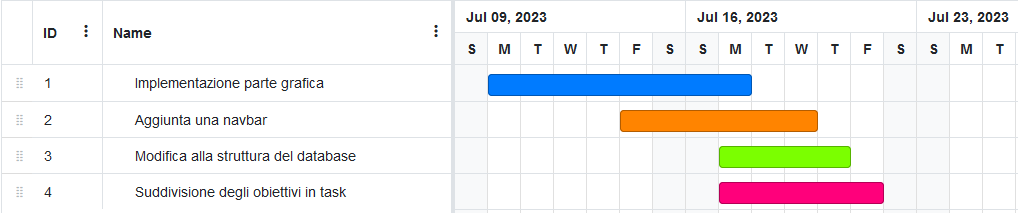
\includegraphics[scale = 0.5]{./res/img/Sprint_4.png}
  \end{center}
\begin{itemize}
    \item \textbf{Durata:} 10/07/2023 - 21/07/2023 
    \item \textbf{Attività svolte:}
    \begin{itemize}
        \item La parte grafica prima implementata su un branch a parte è stata implementata anche sull'applicativo issuer;
        \item Assieme alla parte grafica è stata aggiunta una navbar nell'applicativo issuer; 
        \item Il database ha subito delle modifiche in particolare alcuni campi oltre che cambiare nome hanno cambiato valori registrati;
        \item I macro obiettivi che volevamo raggiungere sono stati suddivisi in task più piccoli da gestire per il gruppo e per i componenti singoli.
    \end{itemize}
    \item \textbf{Difficoltà riscontrate:}
    \item \textbf{Costi Previsti:}
    \begin{longtable}{|c|c|c|c|}
        \hline
        Ruolo & Descrizione & Ore & Costo \\
        \hline
        RE & Responsabile & 2 & 60€ \\
        \hline
        AN & Analista & 2 & 50€ \\
        \hline
        VE & Verificatore & 2 & 40€ \\
        \hline
        PR & Programmatore & 16 & 240€ \\
        \hline
        PT & Progettista & 8 & 200€ \\
        \hline
        AM & Amministratore & 8 & 160€ \\
        \hline
        Totale & & 38 & 750€ \\
        \hline
        \end{longtable}
    \item \textbf{Costi effettivi:}
    \begin{longtable}{|p{0.1\textwidth}|c|c|c|c|c|c|c|c|}
        \hline
        Nome & RE & AN & VE & PR & PT & AM & Ore & Costi\\
        \hline
        Ibra \newline Elton & &2 & &3 &3 & &8 & 170€\\
        \hline
        Beschin Michele &2 & & &5 & & &7 & 135€\\
        \hline
        Lotto \newline Riccardo & & &3 &4 & & &7 & 120€\\
        \hline
        Bobirica Andrei Cristian & & & &5 & & &5 & 75€\\
        \hline
        Andreetto Alessio & &1 & & &5 & &6 & 150€\\
        \hline
        Corbu Teodor Mihail & & & & & &7 &7 & 140€\\
        \hline
        Totale &2 &3 &3 &17 &8 &7 &40 & 790€\\
        \hline
    \end{longtable}
    \end{itemize}